\documentclass[journal,12pt,twocolumn]{IEEEtran}

\usepackage{setspace}
\usepackage{gensymb}
\singlespacing
\usepackage[cmex10]{amsmath}

\usepackage{amsthm}

\usepackage{mathrsfs}
\usepackage{txfonts}
\usepackage{stfloats}
\usepackage{bm}
\usepackage{cite}
\usepackage{cases}
\usepackage{subfig}

\usepackage{longtable}
\usepackage{multirow}

\usepackage{enumitem}
\usepackage{mathtools}
\usepackage{steinmetz}
\usepackage{tikz}
\usepackage{circuitikz}
\usepackage{verbatim}
\usepackage{tfrupee}
\usepackage[breaklinks=true]{hyperref}
\usepackage{graphicx}
\usepackage{tkz-euclide}

\usetikzlibrary{calc,math}
\usepackage{listings}
    \usepackage{color}                                            %%
    \usepackage{array}                                            %%
    \usepackage{longtable}                                        %%
    \usepackage{calc}                                             %%
    \usepackage{multirow}                                         %%
    \usepackage{hhline}                                           %%
    \usepackage{ifthen}                                           %%
    \usepackage{lscape}     
\usepackage{multicol}
\usepackage{chngcntr}
\usepackage{textcomp}
\usepackage{float}
\restylefloat{table}

\DeclareMathOperator*{\Res}{Res}

\renewcommand\thesection{\arabic{section}}
\renewcommand\thesubsection{\thesection.\arabic{subsection}}
\renewcommand\thesubsubsection{\thesubsection.\arabic{subsubsection}}

\renewcommand\thesectiondis{\arabic{section}}
\renewcommand\thesubsectiondis{\thesectiondis.\arabic{subsection}}
\renewcommand\thesubsubsectiondis{\thesubsectiondis.\arabic{subsubsection}}


\hyphenation{op-tical net-works semi-conduc-tor}
\def\inputGnumericTable{}                                 %%

\lstset{
%language=C,
frame=single, 
breaklines=true,
columns=fullflexible
}
\begin{document}

\newcommand{\BEQA}{\begin{eqnarray}}
        \newcommand{\EEQA}{\end{eqnarray}}
\newcommand{\define}{\stackrel{\triangle}{=}}
\bibliographystyle{IEEEtran}
\raggedbottom
\setlength{\parindent}{0pt}
\providecommand{\mbf}{\mathbf}
\providecommand{\pr}[1]{\ensuremath{\Pr\left(#1\right)}}
\providecommand{\qfunc}[1]{\ensuremath{Q\left(#1\right)}}
\providecommand{\sbrak}[1]{\ensuremath{{}\left[#1\right]}}
\providecommand{\lsbrak}[1]{\ensuremath{{}\left[#1\right.}}
\providecommand{\rsbrak}[1]{\ensuremath{{}\left.#1\right]}}
\providecommand{\brak}[1]{\ensuremath{\left(#1\right)}}
\providecommand{\lbrak}[1]{\ensuremath{\left(#1\right.}}
\providecommand{\rbrak}[1]{\ensuremath{\left.#1\right)}}
\providecommand{\cbrak}[1]{\ensuremath{\left\{#1\right\}}}
\providecommand{\lcbrak}[1]{\ensuremath{\left\{#1\right.}}
\providecommand{\rcbrak}[1]{\ensuremath{\left.#1\right\}}}
\theoremstyle{remark}
\newtheorem{rem}{Remark}
\newcommand{\sgn}{\mathop{\mathrm{sgn}}}
\providecommand{\abs}[1]{\vert#1\vert}
\providecommand{\res}[1]{\Res\displaylimits_{#1}}
\providecommand{\norm}[1]{\lVert#1\rVert}
%\providecommand{\norm}[1]{\lVert#1\rVert}
\providecommand{\mtx}[1]{\mathbf{#1}}
\providecommand{\mean}[1]{E[#1]}
\providecommand{\fourier}{\overset{\mathcal{F}}{ \rightleftharpoons}}
%\providecommand{\hilbert}{\overset{\mathcal{H}}{ \rightleftharpoons}}
\providecommand{\system}{\overset{\mathcal{H}}{ \longleftrightarrow}}
%\newcommand{\solution}[2]{\textbf{Solution:}{#1}}
\newcommand{\solution}{\noindent \textbf{Solution: }}
\newcommand{\cosec}{\,\text{cosec}\,}
\newcommand{\comb}[2]{{}^{#1}\mathrm{C}_{#2}}
\providecommand{\dec}[2]{\ensuremath{\overset{#1}{\underset{#2}{\gtrless}}}}
\newcommand{\myvec}[1]{\ensuremath{\begin{pmatrix}#1\end{pmatrix}}}
\newcommand{\mydet}[1]{\ensuremath{\begin{vmatrix}#1\end{vmatrix}}}
\numberwithin{equation}{subsection}
\makeatletter
\@addtoreset{figure}{problem}
\makeatother
\let\StandardTheFigure\thefigure
\let\vec\mathbf
\renewcommand{\thefigure}{\theproblem}
\def\putbox#1#2#3{\makebox[0in][l]{\makebox[#1][l]{}\raisebox{\baselineskip}[0in][0in]{\raisebox{#2}[0in][0in]{#3}}}}
\def\rightbox#1{\makebox[0in][r]{#1}}
\def\centbox#1{\makebox[0in]{#1}}
\def\topbox#1{\raisebox{-\baselineskip}[0in][0in]{#1}}
\def\midbox#1{\raisebox{-0.5\baselineskip}[0in][0in]{#1}}
\vspace{3cm}
\title{AI1103 Assignment-8}
\author{SRIVATSAN T - CS20BTECH11062}
\maketitle
\newpage
\bigskip
\renewcommand{\thefigure}{\theenumi}
\renewcommand{\thetable}{\theenumi}
Download all python codes from
\begin{lstlisting}
https://github.com/CS20BTECH11062/AI1103/tree/main/Assignment-8/codes
\end{lstlisting}
%
and latex-tikz codes from
%
\begin{lstlisting}
https://github.com/CS20BTECH11062/AI1103/tree/main/Assignment-8/Assignment-8.tex
\end{lstlisting}
\section*{QUESTION\\(UGC MATH (mathA) June 2017 Q.52)}
X and Y are independent random variables each having the density
\begin{align}
    f(t) = \displaystyle\frac{1}{\pi} \frac{1}{1+{t}^2} -\infty < t < +\infty
\end{align}
Then the density function of $\displaystyle\frac{X+Y}{3}$ for \\$-\infty <$ t $< +\infty$ is\bigskip
    \begin{enumerate}\itemsep0.5cm
        \item $\displaystyle\frac{6}{\pi} \frac{1}{4+9{t}^2}$
        \item $\displaystyle\frac{6}{\pi} \frac{1}{9+4{t}^2}$
        \item $\displaystyle\frac{3}{\pi} \frac{1}{1+9{t}^2}$
        \item $\displaystyle\frac{3}{\pi} \frac{1}{9+{t}^2}$
    \end{enumerate}
    \section*{SOLUTION}
    Let us consider the random variables X and Y.
    The Characteristic function of the probability density $f(t)$ is
    \begin{align}
        g(w) =\hspace{0.2cm} & \int_{-\infty}^{\infty}  f(t) {e}^{iwt} dt                                         \\[0.2cm]
        =\hspace{0.2cm}      & \int_{-\infty}^{\infty}  \displaystyle\frac{1}{\pi} \frac{1}{1+{t}^2} {e}^{iwt} dt \\[0.2cm]
        =\hspace{0.2cm}      & e^{-\abs{w}}\hspace{0.2cm}, -\infty<w<\infty
    \end{align}
    The product of the Characteristic function of \\probability density of X and Y is
    \begin{align}
        h(w) = g_1(w) \times g_2(w) = {e}^{-2\abs{w}}
    \end{align}
    To get the probability density of X+Y, we find the inverse characteristic function of h(w).
    \begin{align}
        F_{X+Y}(t) =\hspace{0.2cm} & \int_{-\infty}^{\infty} h(w) {e}^{-iwt} dw           \\[0.2cm]
        =\hspace{0.2cm}            & \int_{-\infty}^{\infty} {e}^{-iwt-2\abs{w}} dw       \\[0.2cm]
        =\hspace{0.2cm}            & \frac{4}{4 + {t}^2} \hspace{0.2cm}, -\infty<t<\infty
    \end{align}
    But since $F_{X+Y}$ is a probability distribution function,\\[0.2cm]$\displaystyle\int_{-\infty}^{\infty} F_{X+Y}(t) dt= 1$.
    \begin{align}
        \text{But}\hspace{0.2cm} \int_{-\infty}^{\infty} F_{X+Y}(t) dt = \int_{-\infty}^{\infty} \frac{4}{4+{t^2}} dt= 2\pi
    \end{align}
    So we plug in the normalisation factor $\displaystyle\frac{1}{2\pi}$ and the new $F_{X+Y}$ becomes
    \begin{align}
        F_{X+Y}(t) = \frac{2}{\pi} \frac{1}{4+{t}^2}\hspace{0.2cm}, -\infty<t<\infty
    \end{align}
    We know that if a random variable M has a\\probability density $f_M(x)$, then the probability \\density of random variable kM is
    \begin{align}
        f_{kM}\brak{x} = \frac{1}{\abs{k}} f_M\brak{\frac{x}{\abs{k}}}
    \end{align}
    Probability density of $Z = \displaystyle\frac{X+Y}{3}$ given $F_{X+Y}(t)$ is
\begin{align}
    F_{Z}(t) = & 3\times \displaystyle f_{X+Y}(3t) \\
    =          & \frac{6}{\pi} \frac{1}{4+9{t}^2}
\end{align}
\begin{center}
    Correct Option : 1
\end{center}
\begin{figure}[H]
    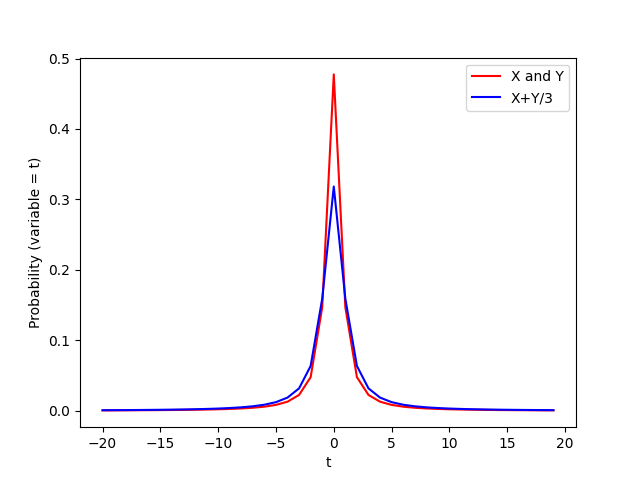
\includegraphics[width = \columnwidth]{Assignment-8.png}
    \caption{Grphs showing initial and convoluted probability densities.Area under both the curves = 1}
\end{figure}
\end{document}